\documentclass[a4paper,12pt]{article} % добавить leqno в [] для нумерации слева
\usepackage[a4paper,top=1.3cm,bottom=2cm,left=1.5cm,right=1.5cm,marginparwidth=0.75cm]{geometry}
%%% Работа с русским языком
\usepackage{cmap}					% поиск в PDF
\usepackage[warn]{mathtext} 		% русские буквы в фомулах
\usepackage[T2A]{fontenc}			% кодировка
\usepackage[utf8]{inputenc}			% кодировка исходного текста
\usepackage[english,russian]{babel}	% локализация и переносы
\usepackage{physics}
\usepackage{multirow}
\usepackage{bm}
\usepackage{longtable}
\usepackage{xcolor}
%%% Нормальное размещение таблиц (писать [H] в окружении таблицы)
\usepackage{float}
\restylefloat{table}


\documentclass[a4paper,12pt]{article}
\usepackage[utf8]{inputenc}
\usepackage[russian]{babel}
\usepackage{amsmath}
\usepackage{amssymb}
\usepackage{graphicx}
\usepackage{geometry}
\usepackage{booktabs}
\usepackage{caption}
\usepackage{enumitem}
\usepackage{siunitx}

\geometry{left=2cm,right=1.5cm,top=2cm,bottom=2cm}
\setlist[enumerate]{label=\arabic*., leftmargin=*}


\usepackage{graphicx}

\usepackage{wrapfig}
\usepackage{tabularx}

\usepackage{hyperref}
\usepackage[rgb]{xcolor}
\hypersetup{
	colorlinks=true,urlcolor=blue
}
\usepackage{pgfplots}
\pgfplotsset{compat=1.9}
%%% Дополнительная работа с математикой
\usepackage{amsmath,amsfonts,amssymb,amsthm,mathtools} % AMS
\usepackage{icomma} % "Умная" запятая: $0,2$ --- число, $0, 2$ --- перечисление

%% Номера формул
%\mathtoolsset{showonlyrefs=true} % Показывать номера только у тех формул, на которые есть \eqref{} в тексте,

%% Шрифты
\usepackage{euscript}	 % Шрифт Евклид
\usepackage{mathrsfs} % Красивый матшрифт

\title{Архитектура вычислительных систем. Домашнее задание №3. Вариант №1.}
\author{Комиссаров Данил Андреевич}
\date{March 2025}

\begin{document}

\maketitle

\section{Полный отчет}
Первый вариант задания. Программа на RISC-V ассемблере.

Здесь будем работать с инструкциями ассемблера RISC-V. Теперь не придётся заниматься проектированием железа, но разбираться с устройством работы моделей предсказаний. Что само по себе является достаточно обширной темой. Предисловия не будет, со всеми темами будем разбираться на местах. 

Это должно быть интересно.

\subsection*{Пункт 1}

Выдан код на ассемблере
\begin{figure}[H]
    \centering
    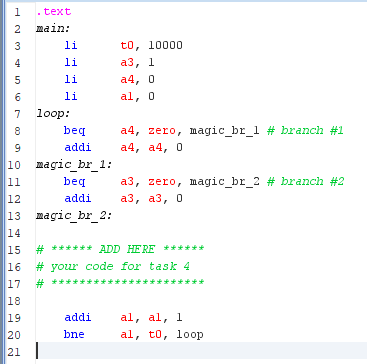
\includegraphics[width=0.5\linewidth]{Part1/code.png}
\end{figure}
Удобно, что при наведении на команду подсвечивается её значение:
\begin{enumerate}
    \item \textbf{li      t0, 10000} - Load Immediate - загрузить 10000 в t0, то есть просто запись констант в регистры
    \item \textbf{beq     a4, zero, magic\_br\_1} - Branch if EQual - прыгнуть по метке magic\_br\_1 если a4 == zero (то есть равенство регистра a4 нулю), то есть команда означает, если первый операнд равен второму, то происходит прыжок по метке, записанной третьим параметром.
    \item \textbf{addi    a4, a4, 0} - ADDiotion Immediate - то есть назначить первому операнду значению, равное сумме второго и третьего, вторым операндом может быть знаковый регистр, а третьим immediate (то есть так называемый непосредственный, далее все immediate будем называть \textit{константы}. Их значения доступны непосредственно из инструкции и не требуют доступа к регистру или памяти).
    \item \textbf{nop} - No OPeration - операция, которая заставляет просто стоять в холостую данный такт. Иногда заменяется на
\[\textit{addi    a0, a0, 0}\]
то есть инструкция-затычка.
    \item \textbf{bne     a1, t0, loop} - Branch if Not Equal - то же самое, что и \textit{beq}, но вместо условия равенства, стоит условие неравенства.
\end{enumerate}
Вроде все понятно, конечно, этот материал пересекается с вторым семестром информатики и изучения ассемблера x86, поэтому особых вопросов возникнуть не должно.

Теперь можно пристальнее присмотреться к коду и заметить, что он выполняет довольно странные действия (впрочем, очевидно, что такой искусственный код написан только для оперирования с модулем предсказания).

А в частности то, что цикл \textbf{loop} выполняется 10000 раз, внутри которого не меняется ни одна переменная. Переписывая этот код на C, можно представить его так:
\begin{figure}[H]
    \centering
    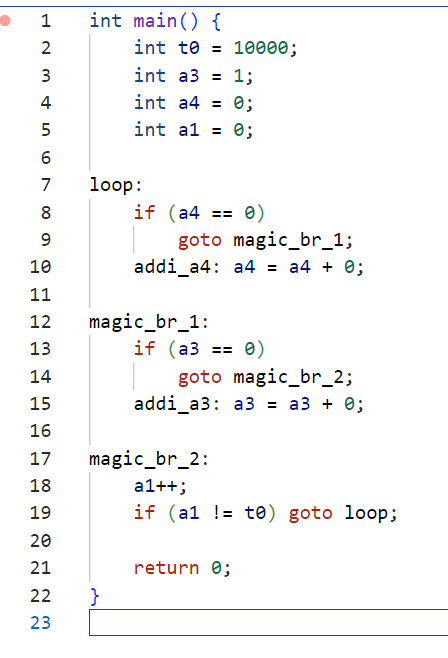
\includegraphics[width=0.5\linewidth]{Part1/c-code.png}
\end{figure}
Понятно, что от этого кода ожидается только вызывать реакцию predict-модуля.

В задании требуется определить точность предсказаний для перехода по magic\_br\_1 и magic\_br\_2. Делая все по инструкции, получаем следующую таблицу:
\begin{figure}[H]
    \centering
    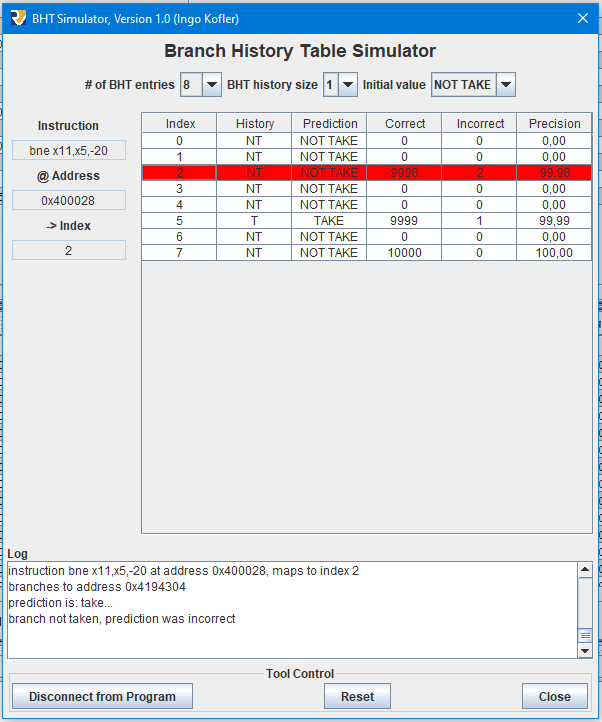
\includegraphics[width=0.5\linewidth]{Part1/BHT.png}
\end{figure}

Интересненько. В задании требуется определить точность предсказаний, но здесь не подписано, какой индекс предиктора соответствует тому или иному условному оператору. Судя по всему, в этом и заключается сложность этого пункта: в сопоставлении этих параметров. 

Можно пойти простым путем и посмотреть в окошке логов, какой адрес инструкции соответствует какому индексу. Или же прокрутить этот код в голове и догадаться, что если значение по-умолчанию - NOT TAKE, то очевидно, что 2 раза угадать неправильно можно было только цикл loop: при входе в него и при выходе, одной ошибке соответствует условный оператор, связанный с меткой magic\_br\_1, и соответственно определить последний условный оператор. Но это слишком просто) Предлагаю посмотреть на эту задачу с другой стороны.

\subsubsection*{Что такое вообще модуль предсказания?}
Очевидно, предсказывает результат условного оператора. Это очень важно для оптимизации работы конвейерных процессоров, сейчас не могу сильно вдаваться в это, и так опаздываю сдать отчет =).

Другой вопрос: как реализовать?
\begin{figure}[H]
    \centering
    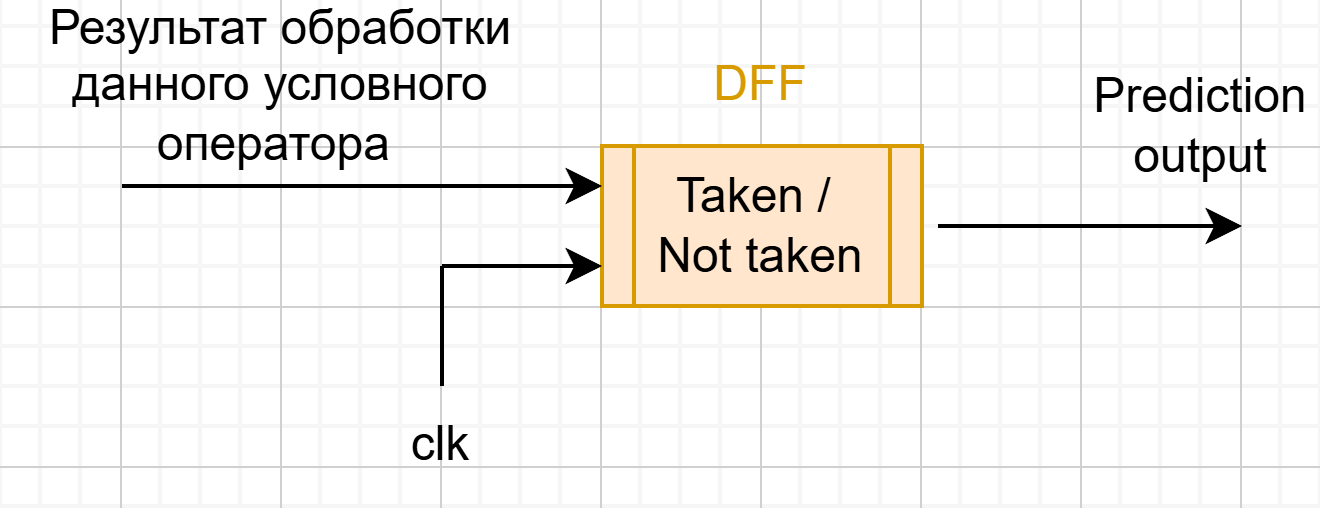
\includegraphics[width=0.75\linewidth]{Part1/predict.png}
\end{figure}
Суть конечного автомата только в том, чтобы сохранить текущее состояние, поэтому его реализацией являются любые ячейки памяти, сохраняющие n бит, в которых зашифровано состояние автомата. В самом простом случае для каждого состояния назначен свой DFF, который сохраняет 1, если автомат работает в этом режиме. Закручено написал, однако...\\

Итак. То есть модуль предсказания - это элемент оптимизации системы на уровне железа, а не на уровне программ. Понятно.\\

Разобрались. Далее: для каждого условного оператора нужно выделить предиктор, но так как это \textit{hardware} оптимизация, то динамически выделить на каждый условный оператор не выйдет: сколько на заводе спаяли модулей предсказания, столько их и будет, что, очевидно, несравнимо меньше, чем условных операторов даже в самой простой программе. 

Поэтому следует их как-то распределять по нескольким операторам на модуль, желательно с наименьшей коллизией. И самый простой способ - это распределение по адресу инструкции, то есть \\
\textit{индекс модуля} = (\textit{номер инструкции} / \textit{размер инструкции}) (mod) \textit{количество модулей}.

Собственно, это можно и проследить в RARS.

\subsubsection*{Выявим принцип распределения модулей}

Возьмем неизменнеую программу из задания и прокомпилируем:
\begin{figure}[H]
    \centering
    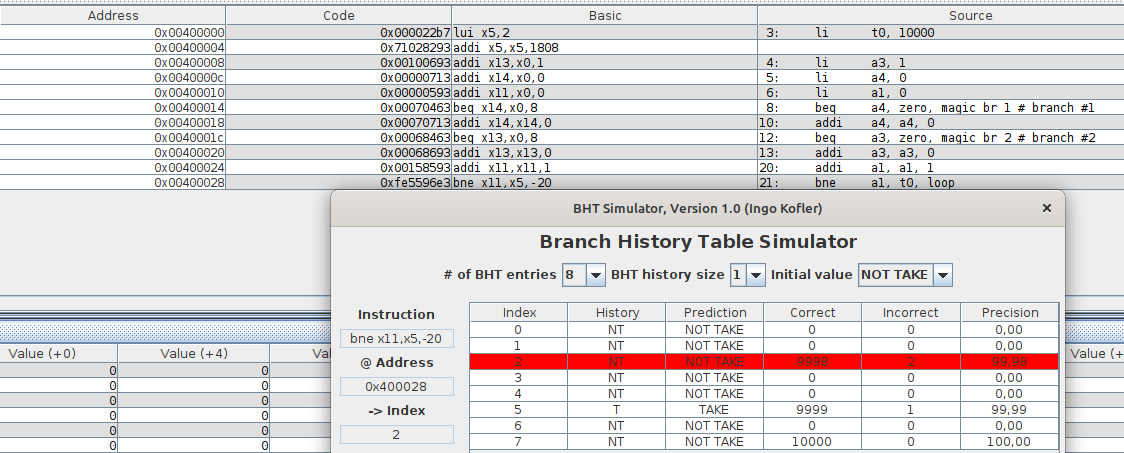
\includegraphics[width=1\linewidth]{Part1/index1.png}
    \caption{Результат отработки неизмененной программы}
\end{figure}

То есть, проверим первый \textbf{beq}, который встречается в коде: он имеет адрес \textit{0x00400014}, длина инструкции составляет \textit{4} байта, а количество модулей \textit{8}:\\
\[0x00400014 / 0x00000004 = 0x00100005\]
\[0x00100005 (mod) 0x00000008 = 0x00000005\]
Вот как получается. Проводя соответствующие вычисления приходим к выводу, что второму \textbf{beq} соответствует индекс \textbf{7}, а инструкции \textbf{bne} - индекс \textbf{2}.

Впрочем. Это ведь всего лишь предположение, что индексы распределяются именно так, может нам просто повезло: но и это можно проверить. Достаточно лишь попередвигать адреса инструкций условных операторов: для того чтобы передвигать адреса, не ломая всю остальную программу идеально подходят, показавшиеся на первый взгляд бесполезными, инструкции \textbf{nop}. 

\begin{figure}[H]
    \centering
    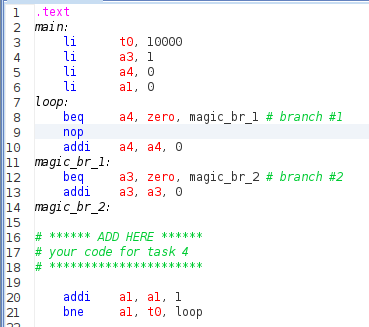
\includegraphics[width=0.5\linewidth]{Part1/nop1.png}
    \caption{Один сдвиг инструкций}
\end{figure}

Вставили один \textbf{nop}, по предположению, последние два условных оператора должны быть назначены модулям с увеличенным на единицу номером, а первый останется на том же месте.

\begin{figure}[H]
    \centering
    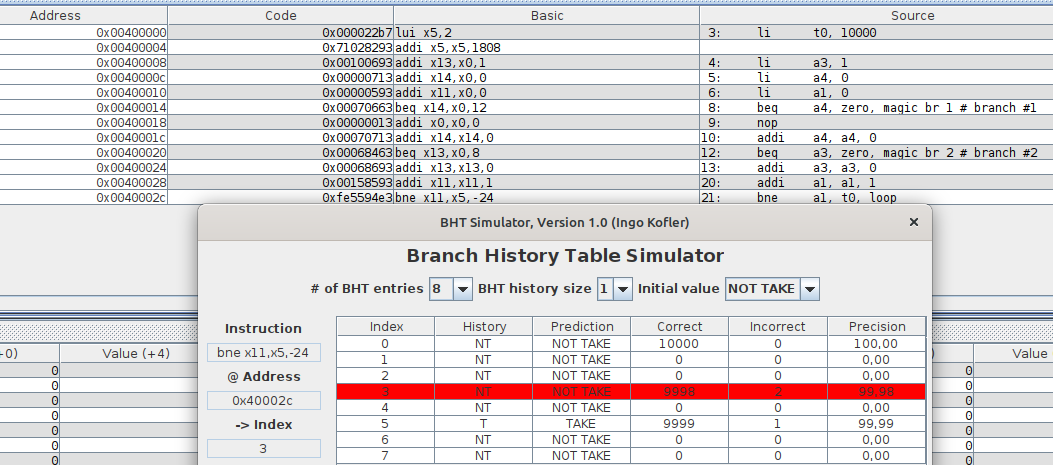
\includegraphics[width=1\linewidth]{Part1/index2.png}
\end{figure}

Действительно. Так и есть, индексы сдвинулись циклически.
Добавляя и другие инструкции и в другие строки, теория подтверждается. \\

Значит, что теперь можем наконец-то с чистой душой смело ответить:

Точность \textbf{bagic\_br\_1} составляет 99,99\%.\\
Точность \textbf{bagic\_br\_2} составляет 100\%.

\begin{figure}[H]
    \centering
    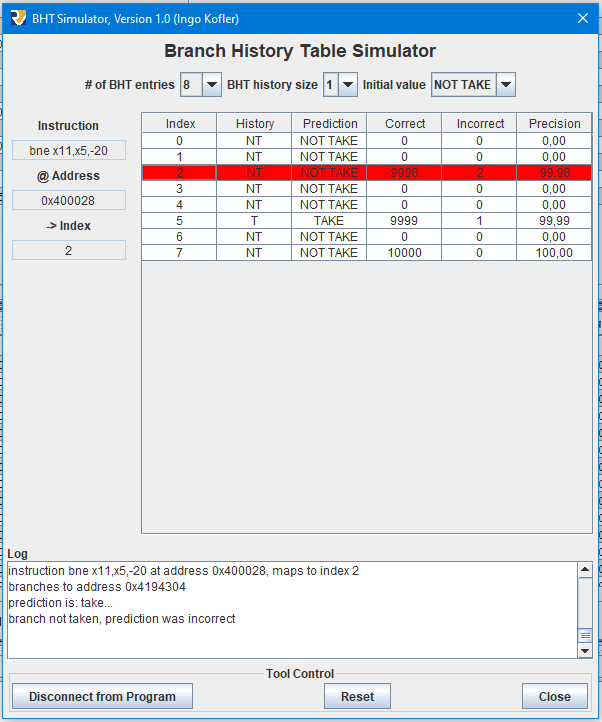
\includegraphics[width=0.5\linewidth]{Part1/BHT.png}
\end{figure}

\subsection*{Пункт 2}

Теперь уже требуется от нас обмануть модуль предсказания. Сейчас в настройках установлен автомат с двумя состояниями, он плохо справляется со случаем, когда результат условного оператора меняется через одного, попеременно выдавая результаты \textit{taken} - \textit{not taken}.

Тогда имеет смысл совместить модули обоих \textbf{beq}, тем более, что уже ранее было выяснено, что первый всегда выдает \textit{taken}, а второй - \textit{not taken}, главное, чтобы сюда не попал третий оператор.

Так и подгоняем их адреса:

\begin{figure}[H]
    \centering
    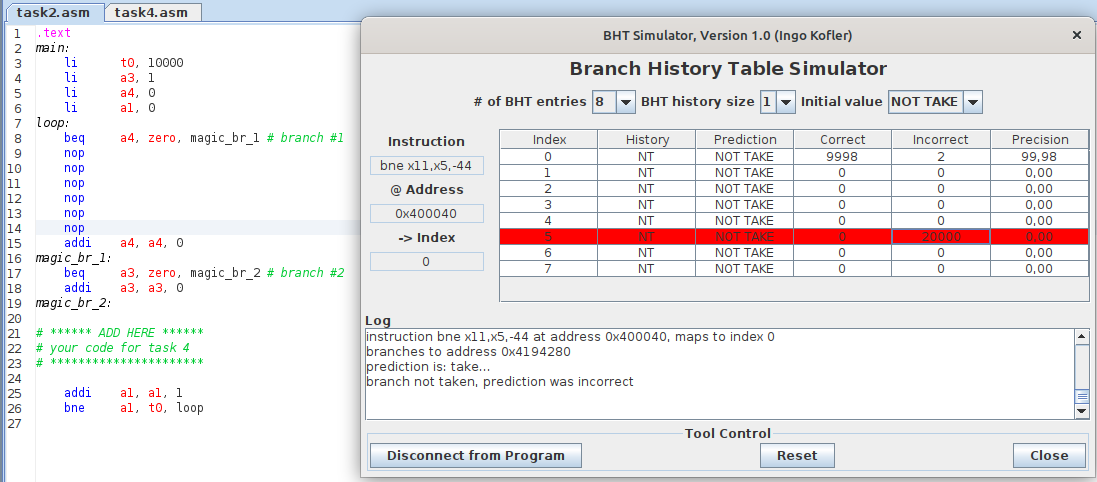
\includegraphics[width=1\linewidth]{Part2/task2.png}
\end{figure}

Впрочем, ничего сложного.
\subsection*{Пункт 3}

Здесь от нас требуется посмотреть на работу конечного автомата с 4 состояниями, который является подвидом бимодального предсказателя.
\begin{figure}[H]
    \centering
    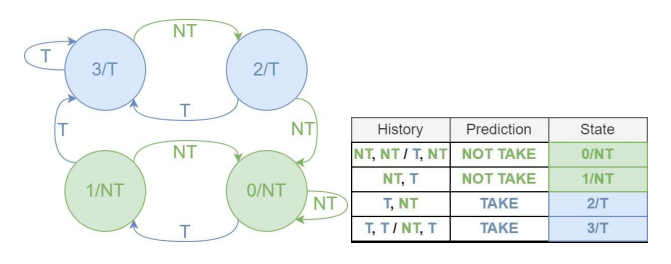
\includegraphics[width=0.75\linewidth]{Part3/bimodal.png}
\end{figure}

Отличается этот от того, что был рассмотрен на лекции тем, что при выходе из \textit{weak taken} переходит сразу в \textit{strong not taken} и наоборот: \textit{weak not taken} -> \textit{strong taken}. Это отличие позволяет не попадаться в ловушку попеременного поведения \textit{taken} - \textit{not taken} - \textit{taken} - \textit{not taken} ...
Выдавая хотябы половину правильных предсказаний, но все же не спасает от \textit{taken} - \textit{taken} - \textit{not taken} - \textit{not taken} ...

От нас требуется лишь посмотреть на его поведение в условиях выше написанной программы:

\begin{figure}[H]
    \centering
    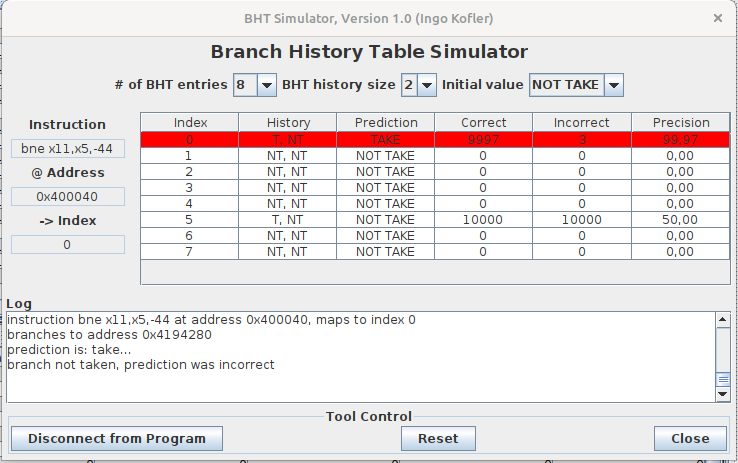
\includegraphics[width=0.75\linewidth]{Part3/BHTbim.png}
\end{figure}

Вот здесь он и выдал в пятом индексе половину правильных предсказаний. \\
Точность - 50\%.

\subsection*{Пункт 4}

Теперь уже требуется обмануть бимодальный предиктор. Впрочему, как это сделать, было описано выше.

Тогда реализуем попеременное поведение инструкций: \textit{taken} - \textit{taken} - \textit{not taken} - \textit{not taken} ...

Так и добьемся 0\% предсказаний.

Разрешено писать только в отведенном месте, но в конце концов на ассемблере пишем, поэтому даже внутри ограниченного пространства можем перелопатить программу до неузнаваемости. 

\begin{figure}[H]
    \centering
    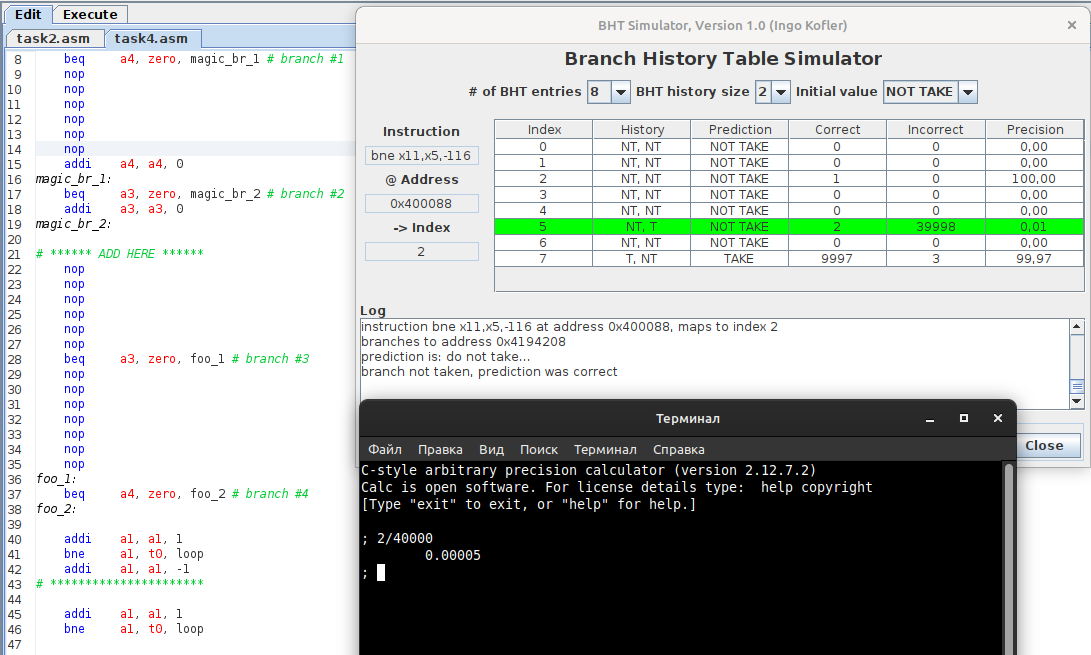
\includegraphics[width=1\linewidth]{Part4/task4.png}
\end{figure}

Здесь подогнали условные операторы так, чтобы специально поломать предиктор, впрочем так и получилось. Процент предсказания уже не прописывается в программе корректно, считаем отдельно в калькуляторе. Увеличивая начальное значение \textbf{t0}, уменьшается процент предсказания, но я не стал увеличивать, так как комп не тянет.

Когда все аспекты рассмотрены, можно начать написание "формального отчета".

\section{Формальный отчет}
\begin{enumerate}
    \item Выполнил: Комиссаров Данил Андреевич.
    \item Студент группы Б01-304.
    \item Первый вариант задания.
    \item Контакты: komissarov.da@phystech.edu
    \item
\end{enumerate}
\begin{enumerate}
    \item 

\begin{figure}[H]
    \centering
    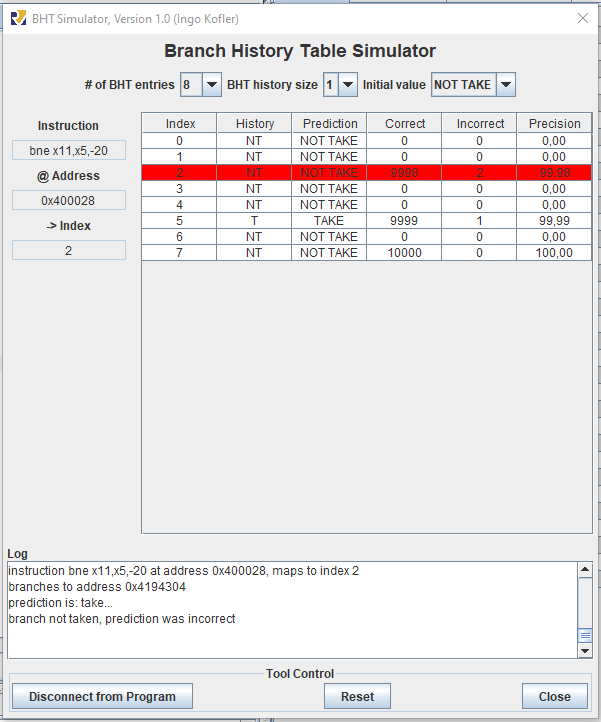
\includegraphics[width=0.75\linewidth]{Formal/BHT1.png}
\end{figure}
Точность \textbf{bagic\_br\_1} составляет 99,99\%.\\
Точность \textbf{bagic\_br\_2} составляет 100\%.
    \item 
\begin{figure}[H]
    \centering
    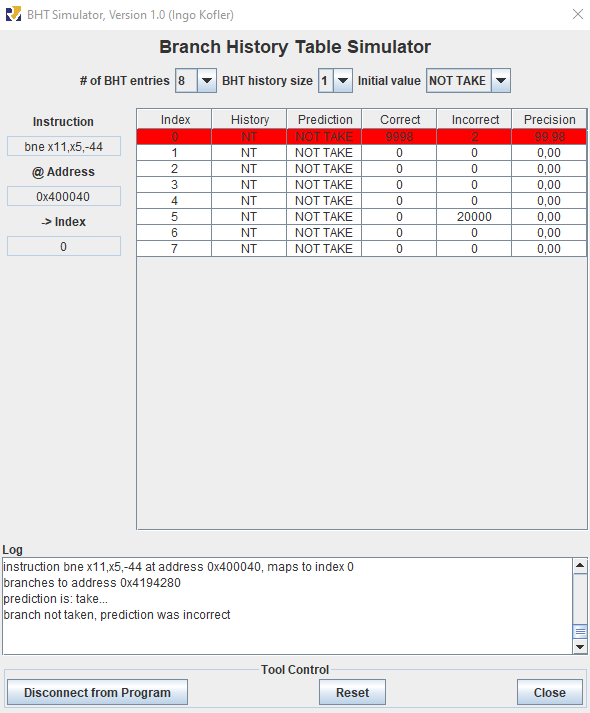
\includegraphics[width=0.75\linewidth]{Formal/BHT2.png}
\end{figure}
\begin{figure}[H]
    \centering
    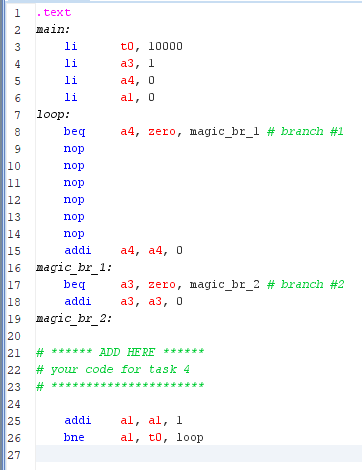
\includegraphics[width=0.5\linewidth]{Formal/task2.png}
\end{figure}
Индексы модулей предсказания для \textbf{beq} \textbf{branch1} и \textbf{branch2} совпали, а так как в настройках предиктора выставлен конечный автомат с двумя состояниями, то обманывать его можно, попеременно выдавая результаты \textit{taken} - \textit{not taken}. Так и добиваемся точности работы предиктора равной нулю.
    \item 
\begin{figure}[H]
    \centering
    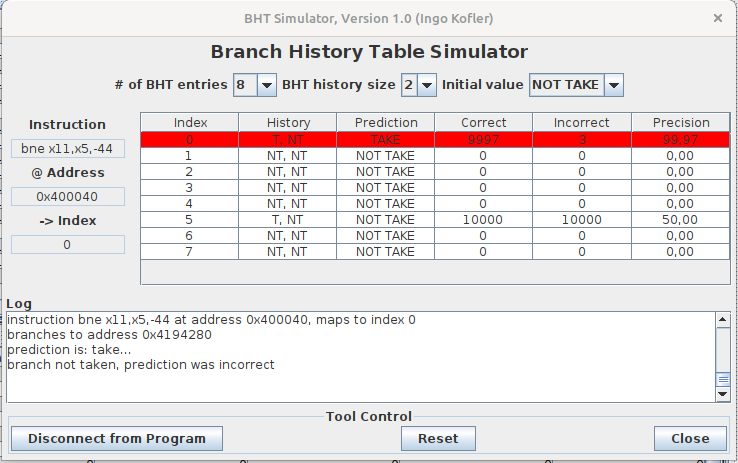
\includegraphics[width=0.75\linewidth]{Formal/BHT3.png}
\end{figure}
В отличие от предиктора из первого задания, сейчас установлен предиктор с 4 состояниями, и причем он построен так, чтобы вместо \textbf{not taken} выдавать \textbf{taken}, необходимо ошибиться 2 раза, что и происходит в цикле \textit{loop}. Так этот предиктор ошибается на 1 раз больше в цикле.
    \item 
\begin{figure}[H]
    \centering
    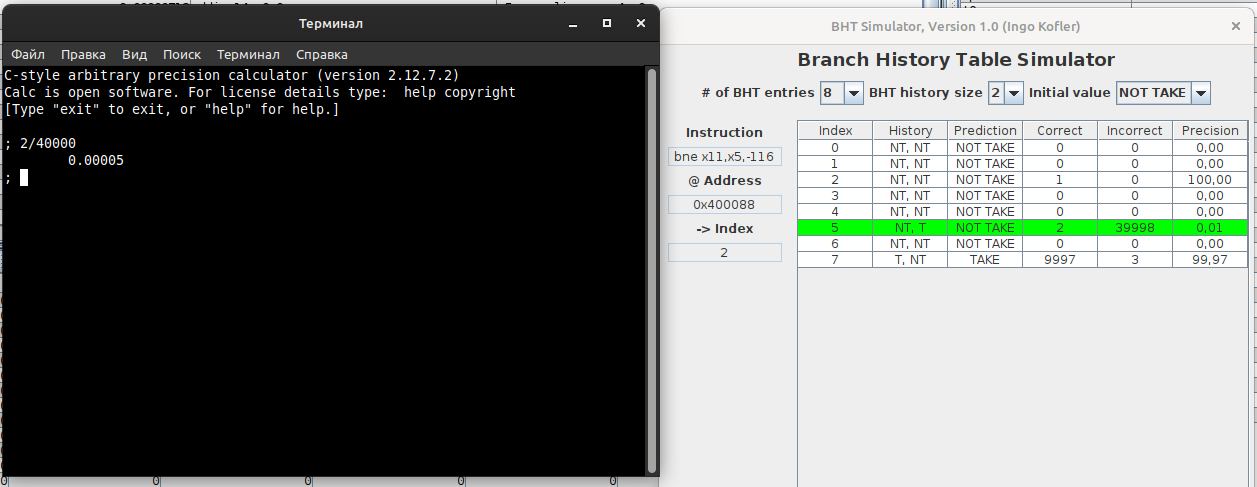
\includegraphics[width=0.75\linewidth]{Formal/BHT4.png}
\end{figure}
\begin{figure}[H]
    \centering
    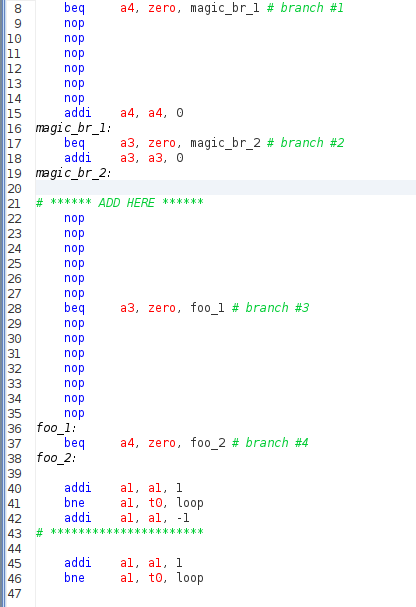
\includegraphics[width=0.75\linewidth]{Formal/task4.png}
\end{figure}
Действительно, так и сделаем: цикл \textbf{taken} - \textbf{taken} - \textbf{not taken} - \textbf{not taken}.
В конце концов на ассемблере пишем, даже внутри ограниченного пространства можем перелопатить программу до неузнаваемости. Корректно процент предсказания уже не прописывается в программе, считаем отдельно в калькуляторе. Увеличивая начальное значение \textbf{t0}, уменьшается процент предсказания, но я не стал увеличивать, так как комп не тянет. 
\end{enumerate}




На этом пожалуй можно и закончить. Наверное я уделил слишком много внимания несущественным аспектам, в то время, когда некоторые фундаментальные принципы были упущены, но это было интересно. 


\end{document}
